\documentclass{article}
\usepackage[utf8]{inputenc}
\title{Actividad 8}
\author{Roberto Alexis Gomez Pintor}
\usepackage{float}
\usepackage{graphicx}
\begin{document}
\maketitle
\section{Introduccion}
La Teoría de Sistemas Dinámicos apareció por primera vez en el siglo XVII al introducir Newton el concepto de ecuaciones diferenciales ordinarias, pero es hasta despues en el siglo XIX que Henri Poincaré se diseña los sistemas dinámicos, seguido por I. Bendixson con el estudio de las propiedades topológicas de las ecuaciones diferenciales ordinarias independientes en el plano. El osciador de Van del Pol modela un circuito eléctrico usado en varias áreas como la biología para las potencialidades de acción de neuronas; la medicina para construir una serie de modelos de circuitos eléctricos del corazón humano para estudiar su rango de estabilidad dinámica; en la matemáticas y física.
\section{Modelo de Van Pol}
\subsection{Historia}
El oscilador de Van del Pol fue propuesto originalmente por el ingeniero eléctrico y físico Balthasar Van del Pol. Van del Pol encontró oscilaciones, llamándolas oscilaciones de relajación, las cuales son conocidas como un tipo de ciclo límite en circuitos eléctricos utilizando tubos de vacío. Cuando estos circuitos se acercan al ciclo límite, la señal envía una corriente con ella. Van del Pol y Van der Mark, el cual era un colega, reportaron que a cierta frecuencias se escuchaba un ruido irregular.
\subsection{Modelo 2 dimensiones}
El Teorema de Liénard puede ser utilizado para ver que el sistema tiene un ciclo límite. Aplicando la transformación de Liénard $y = x - \frac{x^3}{3} - \frac{\dot{x}}{\mu}$  donde el punto representa la primera derivada, el oscilador de Van del Pol puede escribirse en su forma dos dimensional:

\[dot{x} = \mu (x - \frac{x^3}{3}) - y \]
\[\dot{y} = \frac{x}{\mu} \]
Otra forma base comúnmente utilizada en la transformación :
\[\dot{x} = y \]
\[\dot{y} = \mu (1 - x^2 )y - x \]
\section{Apéndice}
\subsection{Este ejercicio pareciera similar al desarrollado en las actividades 6 y 7. ¿Qué aprendiste nuevo?}
Crear códigos a partir de otros para desarrollar mejor los ejercicios.
\subsection{¿Qué fue lo que más te llamó la atención del oscilador de Van der Pol?}
Que no importaba cuanto cambiaras sus condiciones iniciales e incluso el amortiguamiento, su forma no era tan sencillo deformarlo como lo fue con las gráficas de las actividades anteriores.
\subsection{Has escuchado ya hablar de caos. ¿Por qué sería importante estudiar este oscilador?}
No lo había escuchado, hasta el desarrollo de la practica.
\subsection{¿Qué mejorarías en esta actividad?}
Nada de momento.
\subsection{¿Algún comentario adicional antes de dejar de trabajar en Jupyter con Python?}
Nada de mejoría o fallo alguno que recalcar.
\subsection{Cerramos la parte de trabajo con Python ¿Que te ha parecido?}
Bastante bien, me costo bastante adaptarme debido que lo desconocía, pero trabajarlo con las practicas me ayudo a entender mejor y usarlo.
\section{Graficas}
\begin{figure}
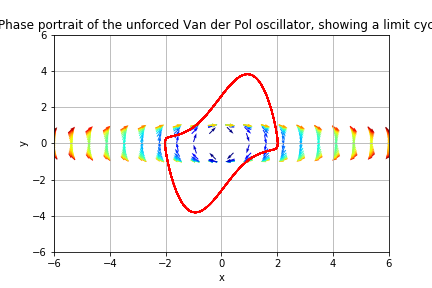
\includegraphics[width=\linewidth]{Image1.png}
\includegraphics[width=\linewidth]{Image1_1.png}
\end{figure}
\begin{figure}
\includegraphics[width=\linewidth]{Image1_2.png}
\includegraphics[width=\linewidth]{Image1_3.png}
\end{figure}
\begin{figure}
\includegraphics[width=\linewidth]{Image1_5.png}
\end{figure}
\begin{figure}
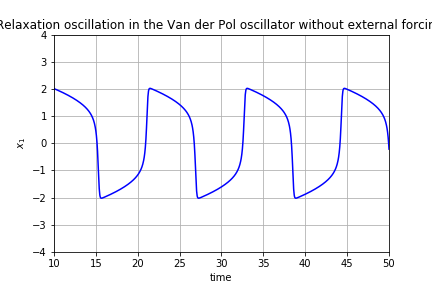
\includegraphics[width=\linewidth]{Image3.png}
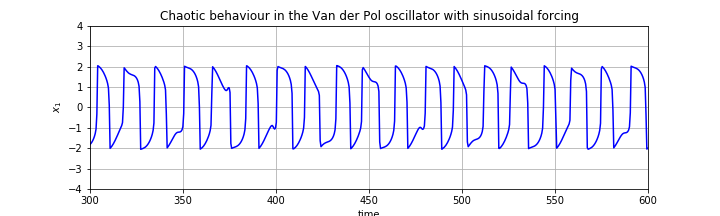
\includegraphics[width=\linewidth]{Image4.png}
\end{figure}
\begin{figure}
\centering
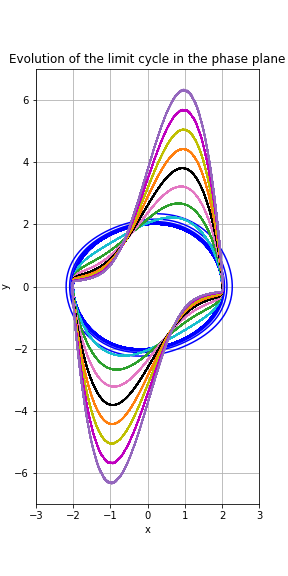
\includegraphics[width=0.5\linewidth]{Image2.png}
\end{figure}
\end{document}